\documentclass[11pt,a4paper]{article}
\usepackage[es-CL]{datetime2}
\DTMsetdatestyle{ddmmyyyy}
\DTMsetup{datesep=/}
\usepackage[utf8]{inputenc}
\usepackage[T1]{fontenc}
\usepackage[left=2.5cm,right=2.5cm,top=2.5cm,bottom=2.5cm]{geometry}
\usepackage{array}
\usepackage{enumitem}
\usepackage{graphicx}
\usepackage{xcolor}
\usepackage{titlesec}
\usepackage{fancyhdr}
\usepackage[most]{tcolorbox}
\usepackage{hyperref}
\usepackage{booktabs}
\usepackage{amsmath}
\usepackage{caption}
\usepackage{subcaption}
\usepackage{multirow}
\renewcommand{\contentsname}{Índice}
\renewcommand{\figurename}{Figura}
\renewcommand{\tablename}{Tabla}
\renewcommand{\refname}{Bibliografía (APA 7)}
\definecolor{negro}{RGB}{0,0,0}
\definecolor{gris}{RGB}{90,90,90}
\definecolor{grisclaro}{RGB}{150,150,150}
\definecolor{fillgray}{RGB}{175,175,175}
\hypersetup{colorlinks=true, linkcolor=negro, urlcolor=negro, citecolor=negro}
\titleformat{\section}{\large\bfseries\color{negro}}{\thesection.}{0.5em}{}
\titleformat{\subsection}{\normalsize\bfseries\color{negro}}{\thesubsection}{0.5em}{}
\titlespacing*{\section}{0pt}{1.3em}{0.4em}
\titlespacing*{\subsection}{0pt}{0.9em}{0.25em}
\pagestyle{fancy}
\fancyhf{}
\fancyfoot[L]{\footnotesize\color{gris}Magíster en Ciencia de Datos e Inteligencia Artificial}
\fancyfoot[R]{\footnotesize\color{gris}\thepage}
\renewcommand{\headrulewidth}{0pt}
\renewcommand{\footrulewidth}{0.4pt}
\captionsetup{font=small,skip=3pt}
\newcommand{\guia}[1]{{\small\itshape\color{gris}#1}\par\vspace{0.15em}}
\newtcolorbox{infobox}[1][Información de la evaluación]{colback=black!3,colframe=negro,
  fonttitle=\bfseries,coltitle=white,title={#1},boxrule=0.6pt,arc=1pt,
  left=7pt,right=7pt,top=4pt,bottom=4pt,breakable}
\newtcolorbox{conexionbox}[1][Conexión con evaluaciones anteriores]{colback=black!6,colframe=gris,
  fonttitle=\bfseries,coltitle=white,title={#1},boxrule=0.6pt,arc=1pt,
  left=7pt,right=7pt,top=4pt,bottom=4pt,breakable}
\newtcolorbox{resultbox}[1][Resultado]{colback=black!4,colframe=grisclaro,
  fonttitle=\bfseries,coltitle=negro,title={#1},boxrule=0.5pt,arc=1pt,
  left=7pt,right=7pt,top=3pt,bottom=3pt,breakable}
\newcommand{\proyTitulo}{Análisis Estadístico de Deserción en Educación Superior}
\newcommand{\proyIntegrantes}{
%
- Pablo Ignacio Balbontín Constenla \\
- Melany Esmeralda Reyes Leiva \\
- Ingeborg Andrea Muñoz Carnot \\
- Mario Alejandro López Pulgar%
}
\newcommand{\proyDataset}{Predict Students' Dropout and Academic Success (UCI, 2022)}
\newcommand{\proyDocente}{Jean Paul Maidana González}
\newcommand{\proyFecha}{\today}
\newcommand{\proyRepo}{\url{https://github.com/dark452/mcdi501-grupo1}}
\setlength{\parindent}{0pt}
\setlength{\parskip}{0.5em}
\begin{document}
\pagenumbering{gobble}
\thispagestyle{empty}
\begin{center}
\vspace*{1.0cm}

\includegraphics[height=4.0cm]{logo_unab.png}\\[1.1cm]
{\footnotesize\color{gris}\MakeUppercase{Magíster en Ciencia de Datos e Inteligencia Artificial}}\\[0.15cm]
{\footnotesize\color{grisclaro}MCDI501: Estadística Computacional para la Toma de Decisiones}\\[1.8cm]
{\Large\bfseries\color{negro} Evaluación Sumativa 2}\\[0.4cm]
{\large\color{negro} Validación mediante Simulación y Remuestreo}\\[0.9cm]
{\small\itshape\color{gris} Informe técnico grupal \textperiodcentered\ Fase 3 del proyecto}
\end{center}
\vspace{1.4cm}
\begin{flushleft}
\setlength{\extrarowheight}{4pt}
\begin{tabular}{@{}>{\bfseries\color{negro}}l l@{}}
Título del proyecto: & \proyTitulo \\
Integrantes:         & \begin{tabular}[t]{@{}l@{}} \proyIntegrantes \end{tabular} \\
Dataset:             & \proyDataset \\
Fase previa:         & Sumativa 1 -- Análisis Exploratorio e Inferencial (Fase 2) \\
Docente:             & \proyDocente \\
Fecha:               & \proyFecha \\
Repositorio GitHub:  & \proyRepo \\
\end{tabular}
\end{flushleft}
\clearpage
\pagenumbering{arabic}
\begin{infobox}
\textbf{Fase del proyecto:} Fase 3: Simulación, Remuestreo y Validación de Robustez\\
\textbf{Modalidad:} Grupal (3-4 integrantes)\qquad\textbf{Puntaje:} 87 pts (según rúbrica)\\
\textbf{Entregables:} Informe PDF \ \textperiodcentered\ Notebook \texttt{.ipynb}\ \textperiodcentered\ Repositorio GitHub\\
\textbf{Resultado de aprendizaje:} validar computacionalmente, mediante simulación y remuestreo, la robustez de los parámetros, pruebas de hipótesis y correlaciones estimadas en la Sumativa 1.
\end{infobox}

\begin{conexionbox}
Este informe no es independiente: retoma explícitamente los resultados de la Sumativa 1
(S1) parámetros e IC (Tabla 3), pruebas de hipótesis (Sección 4) y matriz de correlación
(Figura 5)  y los somete a bootstrap, permutación, simulación Monte Carlo y jackknife para
evaluar su robustez. Semilla fija \texttt{seed=42} en todo el notebook \texttt{F3.ipynb}.
\end{conexionbox}

\vspace{0.3em}
\tableofcontents
\newpage
\section{Validación de resultados de la Sumativa 1 mediante bootstrap}

\begin{conexionbox}
S1 (Sección 3, Tabla 3) estimó IC al 95\,\% para cuatro parámetros mediante la distribución
$t$ de Student. Esta sección remuestrea los mismos datos para validar si esos intervalos son
sensibles al supuesto de normalidad asintótica.
\end{conexionbox}

El método clásico, $\bar{X}\pm t_{\alpha/2,n-1}\cdot s/\sqrt{n}$, asume normalidad asintótica
de la media. Es razonable con $n=4{,}424$, pero cuestionable en variables asimétricas (Edad,
asimetría $+2.05$) o con dependencia por cohortes (PIB, compartido por período de matrícula).
El bootstrap no paramétrico no requiere supuestos distribucionales. Se validan los cuatro
parámetros de S1 con $B=10{,}000$ remuestras, calculando IC \textbf{percentil} y \textbf{BCa}
(\textit{bias-corrected and accelerated}), que corrige sesgo (factor $z_0$) y asimetría
(factor de aceleración $a$, estimado por jackknife), siguiendo Efron y Tibshirani
\cite{efron1993}.

\begin{table}[h!]
\centering
\small
\begin{tabular}{lrrrr}
\toprule
\textbf{Variable} & \textbf{Media} & \textbf{IC clásico (S1)} & \textbf{IC boot. percentil} & \textbf{IC BCa} \\
\midrule
Nota de Admisión        & 126.978 & [126.551, 127.405] & [126.560, 127.402] & [126.558, 127.399] \\
Edad al Matricularse    &  23.265 & [23.041, 23.489]   & [23.050, 23.489]   & [23.055, 23.498] \\
Nota 1\textsuperscript{er} Semestre & 10.641 & [10.498, 10.784] & [10.498, 10.784] & [10.496, 10.783] \\
PIB                     &   0.002 & [$-$0.065, 0.069]  & [$-$0.066, 0.068]  & [$-$0.068, 0.065] \\
\bottomrule
\end{tabular}
\caption{Comparación de intervalos de confianza al 95\,\% ($n=4{,}424$, $B=10{,}000$ remuestras).}
\label{tab:boot_ci}
\end{table}

\begin{figure}[h!]
\centering
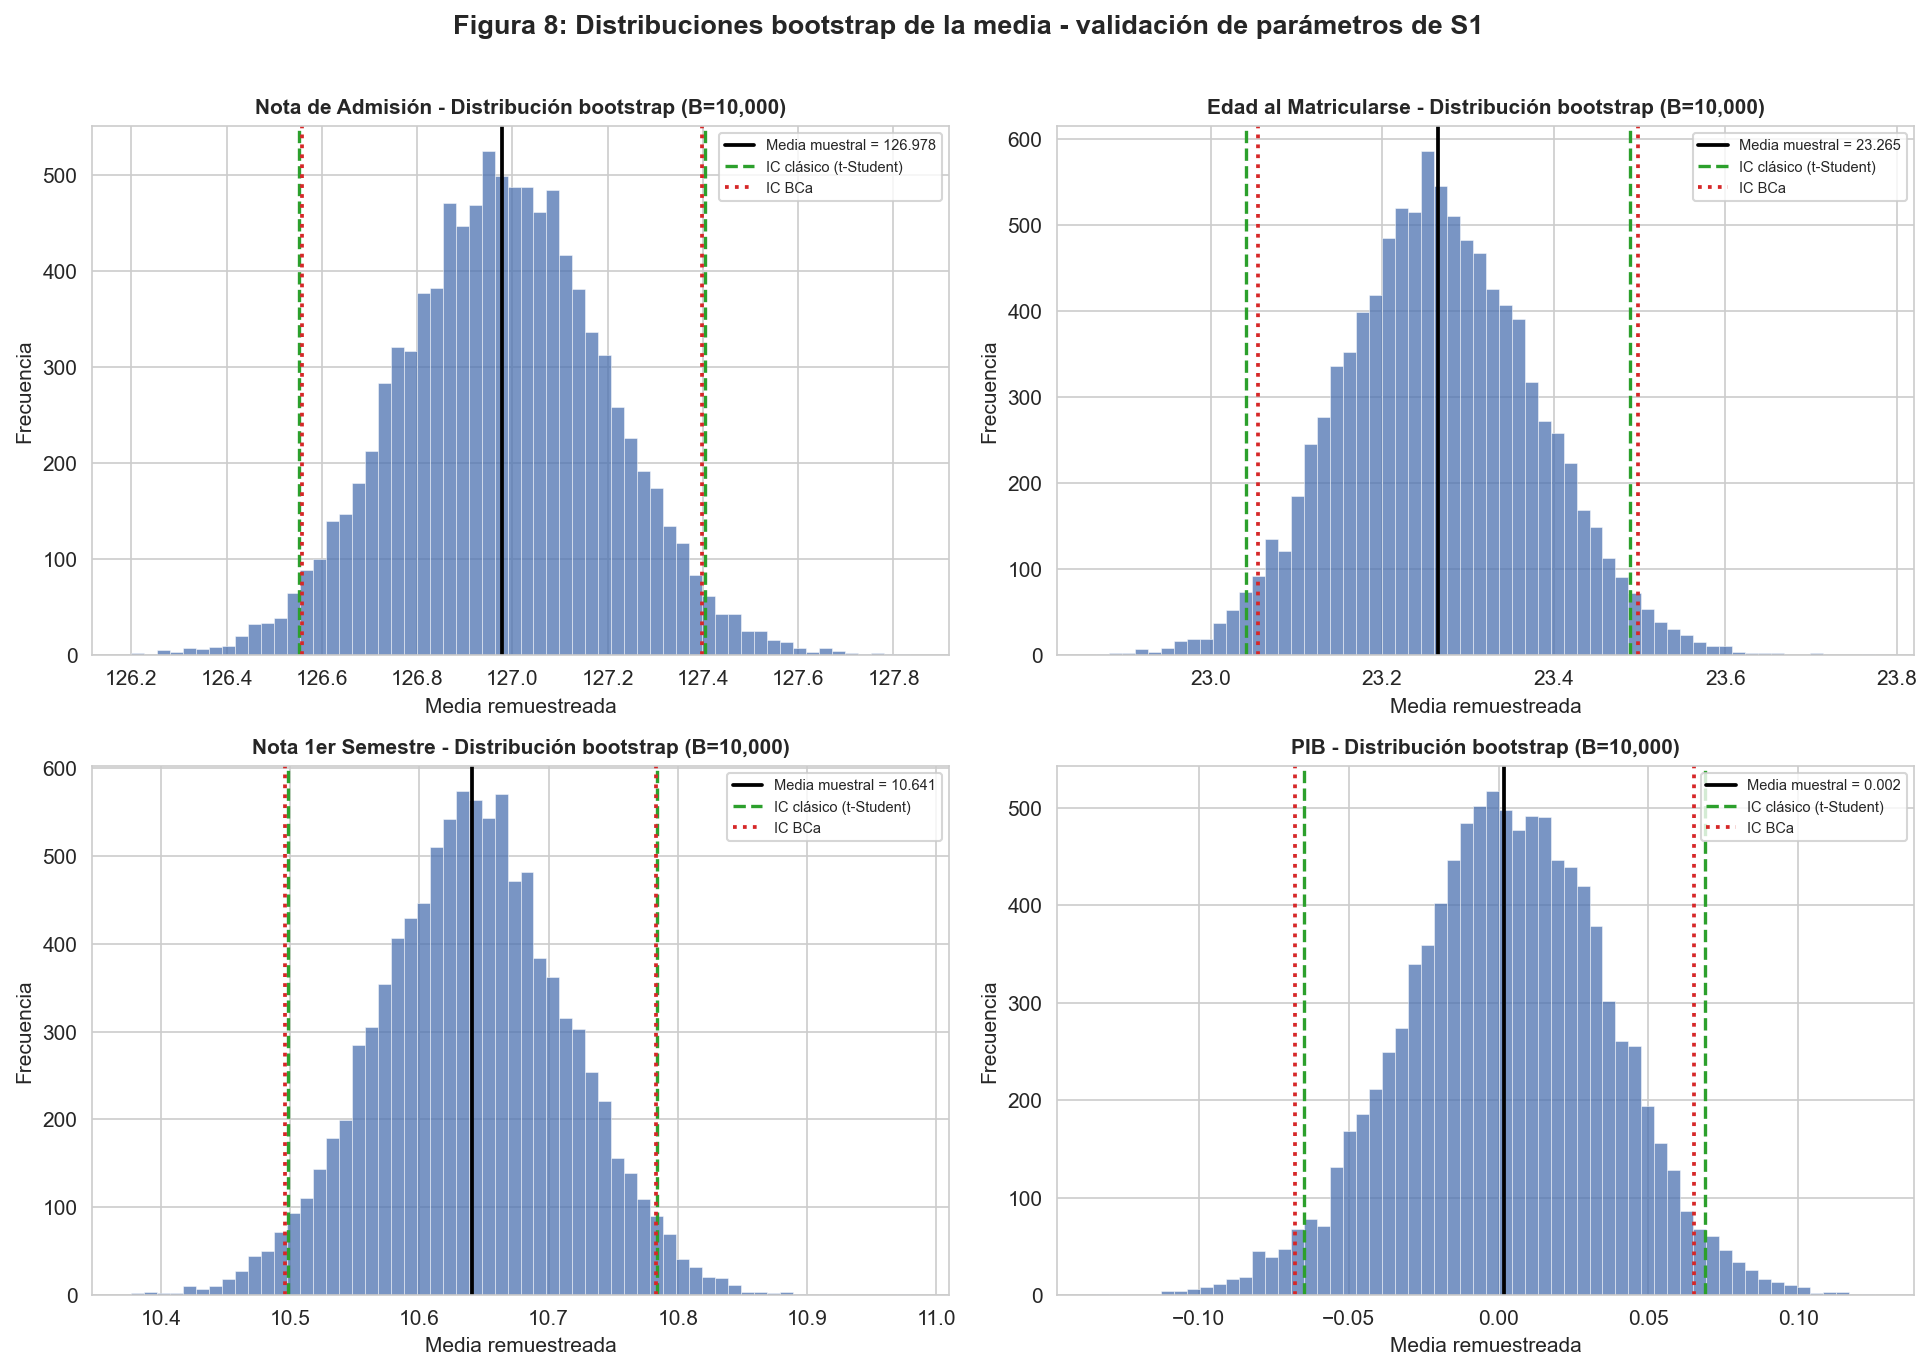
\includegraphics[width=0.95\textwidth]{fig8_bootstrap_parametros.png}
\caption{Distribuciones bootstrap de la media para los cuatro parámetros validados. Verde: IC
clásico de S1; rojo: IC BCa.}
\label{fig:boot}
\end{figure}

Para Nota de Admisión, Nota 1\textsuperscript{er} Semestre y, en menor medida, PIB, los tres
intervalos coinciden hasta la tercera cifra decimal: evidencia empírica de que, con
$n=4{,}424$, el supuesto de normalidad asintótica de S1 era razonable. La \textbf{Edad}, pese
a su asimetría, no muestra discrepancia en la media porque el error de aproximación normal
\emph{en la media} es despreciable a este tamaño muestral; esto no implica que la media sea el
estadístico más representativo del ``estudiante típico'' (ver Sección 5). El \textbf{PIB}
reproduce el hallazgo de S1 (IC incluye el cero), pero el bootstrap \emph{no resuelve} la
limitación estructural ya señalada: al remuestrear con reemplazo sobre las 4{,}424 filas se
sigue tratando como independientes observaciones que comparten valor por cohorte de matrícula,
heredando el mismo sesgo de subestimación del error estándar que el método paramétrico.
Corregir esto exigiría un bootstrap por bloques a nivel de cohorte (recomendación para S3).

\section{Validación de pruebas de hipótesis mediante permutación}

\begin{conexionbox}
S1 (Sección 4) reportó dos pruebas: Prueba 1 ($t$ de Welch, $t=-7.66$, $p<0.001$) y Prueba 2
($\chi^2$, $\chi^2=409.94$, $p<0.001$). Se validan ambas mediante permutación, que no depende
de los supuestos distribucionales parcialmente incumplidos en S1.
\end{conexionbox}

Se valida en detalle la \textbf{Prueba 1}, la más sensible a normalidad: en S1 el grupo
\textit{Graduate} rechazó Shapiro-Wilk ($p=0.011$). El estadístico observado es la diferencia
de medias (\textit{Graduate}$-$\textit{Dropout}); se combinan las 3{,}630 observaciones, se
permutan las etiquetas $10{,}000$ veces y se recalcula la diferencia en cada permutación. Se
extiende el ejercicio a la \textbf{Prueba 2} por su relevancia directa para la Sección 4.

\begin{resultbox}[Resultado - Prueba 1: permutación]
\begin{tabular}{ll}
Diferencia observada (Graduate $-$ Dropout) & 3.833 puntos \\
Estadístico $t$ de Welch (paramétrico)      & $t=-7.657$, $p=2.59\times10^{-14}$ \\
Valor $p$ permutación ($N=10{,}000$)        & $p=1.0\times10^{-4}$ \\
Decisión                                    & \textbf{Rechazar $H_0$} (concuerda con S1) \\
\end{tabular}
\end{resultbox}

\begin{figure}[h!]
\centering
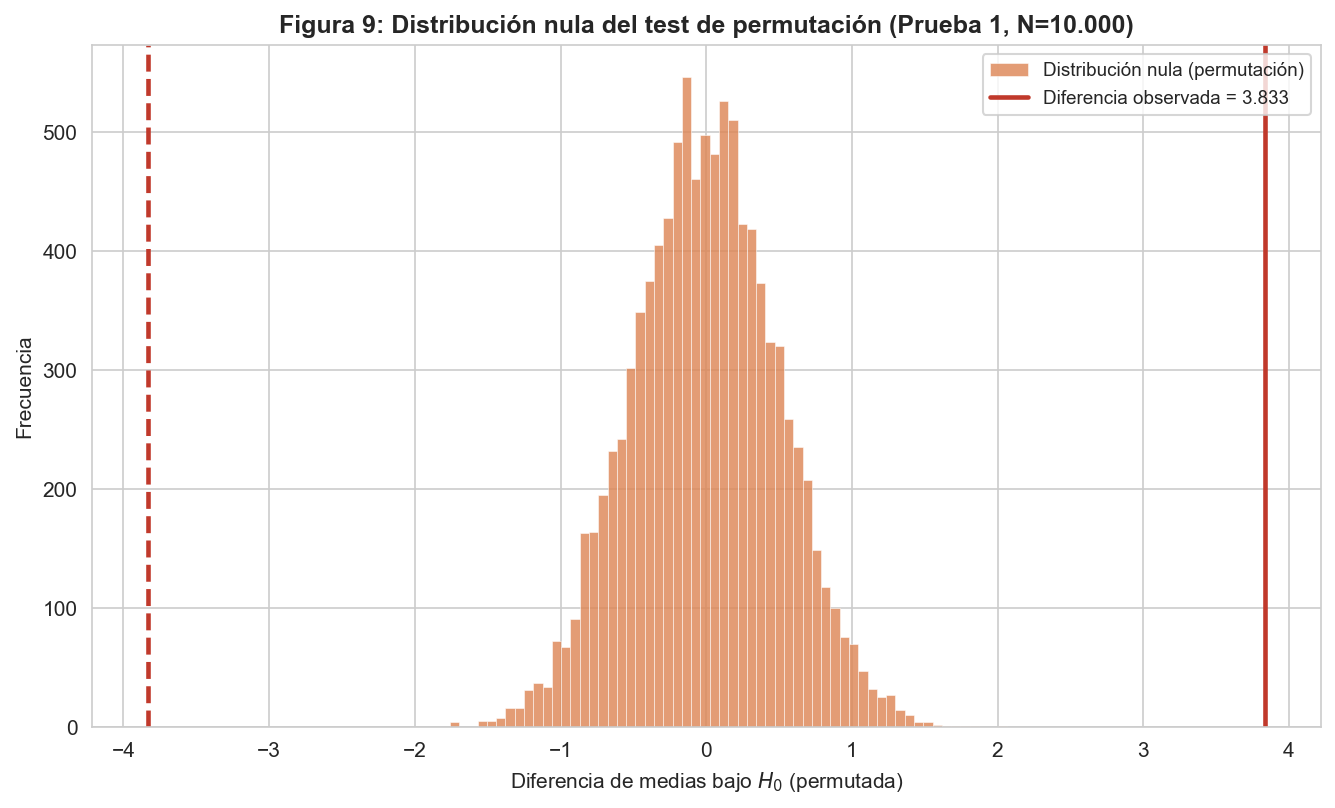
\includegraphics[width=0.85\textwidth]{fig9_permutacion_test1.png}
\caption{Distribución nula del test de permutación, Prueba 1 (10.000 permutaciones).}
\label{fig:perm}
\end{figure}

\begin{resultbox}[Resultado - Prueba 2: permutación (extensión)]
\begin{tabular}{ll}
$\chi^2$ observado (Cramér's $V=0.304$) & 409.943 \\
Valor $p$ paramétrico                   & $9.59\times10^{-90}$ \\
Valor $p$ permutación ($N=10{,}000$)    & $p=1.0\times10^{-4}$ \\
Decisión                                & \textbf{Rechazar $H_0$} (concuerda con S1) \\
\end{tabular}
\end{resultbox}

Ambos valores $p$ de permutación son consistentes con S1 y la decisión de rechazo de $H_0$ es
idéntica bajo ambos marcos inferenciales. Para la Prueba 1, la concordancia casi exacta
confirma que el Teorema Central del Límite ya garantizaba la validez del $t$ de Welch pese a
la violación de normalidad detectada en \textit{Graduate}. Para la Prueba 2, las frecuencias
esperadas mínimas (197.24, muy por encima del umbral de 5) ya garantizaban el cumplimiento de
los supuestos del $\chi^2$; la permutación es aquí una confirmación adicional más que una
corrección. En ambos casos, la evidencia sustantiva del proyecto queda validada con
independencia del marco inferencial elegido.

\section{Evaluación de estabilidad de correlaciones}

\begin{conexionbox}
La matriz de correlación de S1 (Figura 5) identificó a las notas semestrales como los
predictores de mayor correlación con el resultado (r=0.57 y r=0.49) y a las variables
macroeconómicas como marginales (salvo PIB, r=0.044). Esta sección evalúa la estabilidad de
esas correlaciones mediante bootstrap.
\end{conexionbox}

Se seleccionan cinco correlaciones de S1: dos fuertes (notas semestrales), una moderada
(edad), una débil (nota de admisión) y una marginal (PIB, la más cercana a cero reportada en
S1). Para cada una se calcula el IC bootstrap al 95\,\% ($B=10{,}000$) y se evalúa si el
intervalo incluye el cero.

\begin{table}[h!]
\centering
\small
\begin{tabular}{lrrrl}
\toprule
\textbf{Variable} & \textbf{$r$ observado} & \textbf{IC 95\,\% bootstrap} & \textbf{Ancho} & \textbf{¿Incluye 0?} \\
\midrule
Nota 2\textsuperscript{do} Semestre  & 0.567  & [0.544, 0.589]   & 0.045 & No \\
Nota 1\textsuperscript{er} Semestre  & 0.485  & [0.461, 0.508]   & 0.048 & No \\
Edad al Matricularse                 & $-$0.243 & [$-$0.274, $-$0.213] & 0.060 & No \\
Nota de Admisión                     & 0.121  & [0.091, 0.150]   & 0.059 & No \\
PIB                                  & 0.044  & [0.016, 0.073]   & 0.057 & No \\
\bottomrule
\end{tabular}
\caption{Estabilidad bootstrap de correlaciones con el resultado académico codificado.}
\label{tab:corr_boot}
\end{table}

\begin{figure}[h!]
\centering
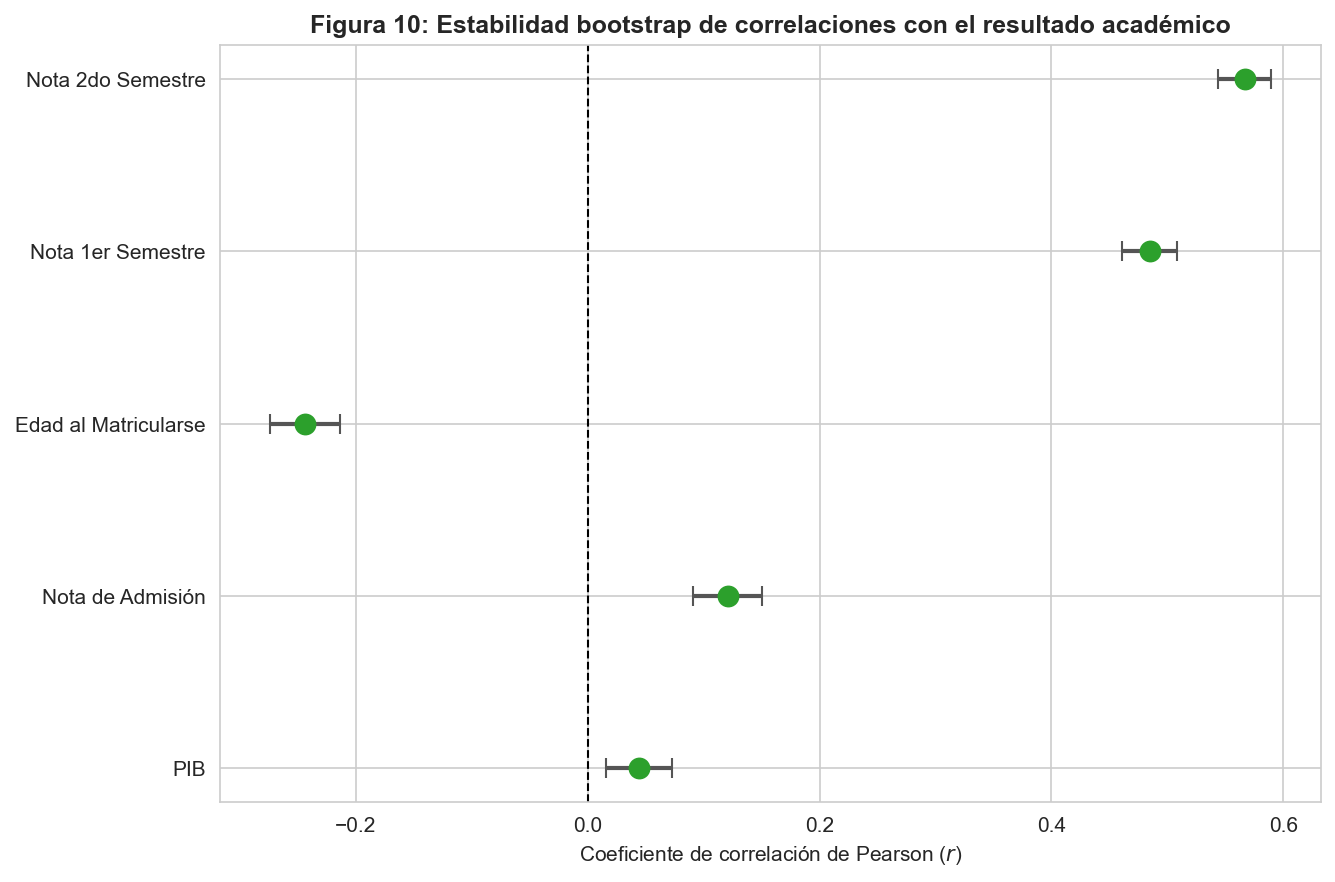
\includegraphics[width=0.9\textwidth]{fig10_estabilidad_correlaciones.png}
\caption{Intervalos de confianza bootstrap al 95\,\% para las cinco correlaciones evaluadas.}
\label{fig:corrboot}
\end{figure}

Las cinco correlaciones presentan intervalos que no incluyen el cero, por lo que en sentido
estrictamente estadístico son ``estables''. No obstante, estabilidad estadística no equivale a
relevancia práctica: las notas semestrales ($r=0.57$ y $r=0.49$, intervalos angostos) son
robustas y de alta relevancia (los predictores más confiables del proyecto); Edad
($r=-0.24$) y Nota de Admisión ($r=0.12$) son robustas pero de relevancia moderada a baja; el
PIB ($r=0.044$) excluye el cero por un margen estrecho y, como se discutió en la Sección 1,
no cumple independencia entre observaciones, por lo que su significancia bootstrap
probablemente está inflada por pseudo-replicación. No debe incorporarse como predictor
individual confiable sin corregir esa estructura de dependencia.

\section{Simulación Monte Carlo basada en parámetros de la Sumativa 1}

\begin{conexionbox}
La Prueba 2 de S1 identificó la beca como el factor externo con mayor asociación práctica
(Cramér's $V=0.30$): los becados se gradúan en 76.0\,\% de los casos frente a 41.3\,\% de los
no becados. S1 concluyó que ampliar la cobertura de becas podría ser una intervención de
retención costo-efectiva, sin cuantificarla. Esta simulación usa exclusivamente los
parámetros de S1 (Tabla 4) para responder esa pregunta.
\end{conexionbox}

\textbf{Diseño}: se simulan cohortes de $n=4{,}424$ estudiantes bajo dos políticas de
cobertura de becas - \emph{base} ($p=24.84\,\%$, observada) y \emph{ampliada} ($p=50\,\%$) -
con $N=10{,}000$ iteraciones cada una. En cada iteración, los resultados académicos de cada
subgrupo se generan mediante muestreo \textbf{multinomial vectorizado} usando las
probabilidades condicionales $P(\text{resultado}\mid\text{beca})$ observadas en S1.

\textbf{Limitación explícita}: se asume que esas probabilidades son transportables a nuevos
becados, ignorando el posible sesgo de selección por motivación ya señalado en S1; el
resultado es, por tanto, un límite superior optimista, no una predicción causal validada.

\begin{table}[h!]
\centering
\small
\begin{tabular}{lrrrr}
\toprule
\textbf{Escenario} & \textbf{Tasa graduación} & \textbf{DE} & \textbf{Tasa deserción} & \textbf{DE} \\
\midrule
Base (cobertura 24.8\,\%)     & 0.4994 & 0.0071 & 0.3212 & 0.0069 \\
Política (cobertura 50.0\,\%) & 0.5864 & 0.0070 & 0.2545 & 0.0063 \\
\midrule
\textbf{Diferencia esperada} & \multicolumn{2}{r}{$+8.71$ p.p.} & \multicolumn{2}{r}{$-6.67$ p.p.} \\
\bottomrule
\end{tabular}
\caption{Resultados de la simulación Monte Carlo ($N=10{,}000$ iteraciones por escenario).}
\label{tab:mc}
\end{table}

\begin{figure}[h!]
\centering
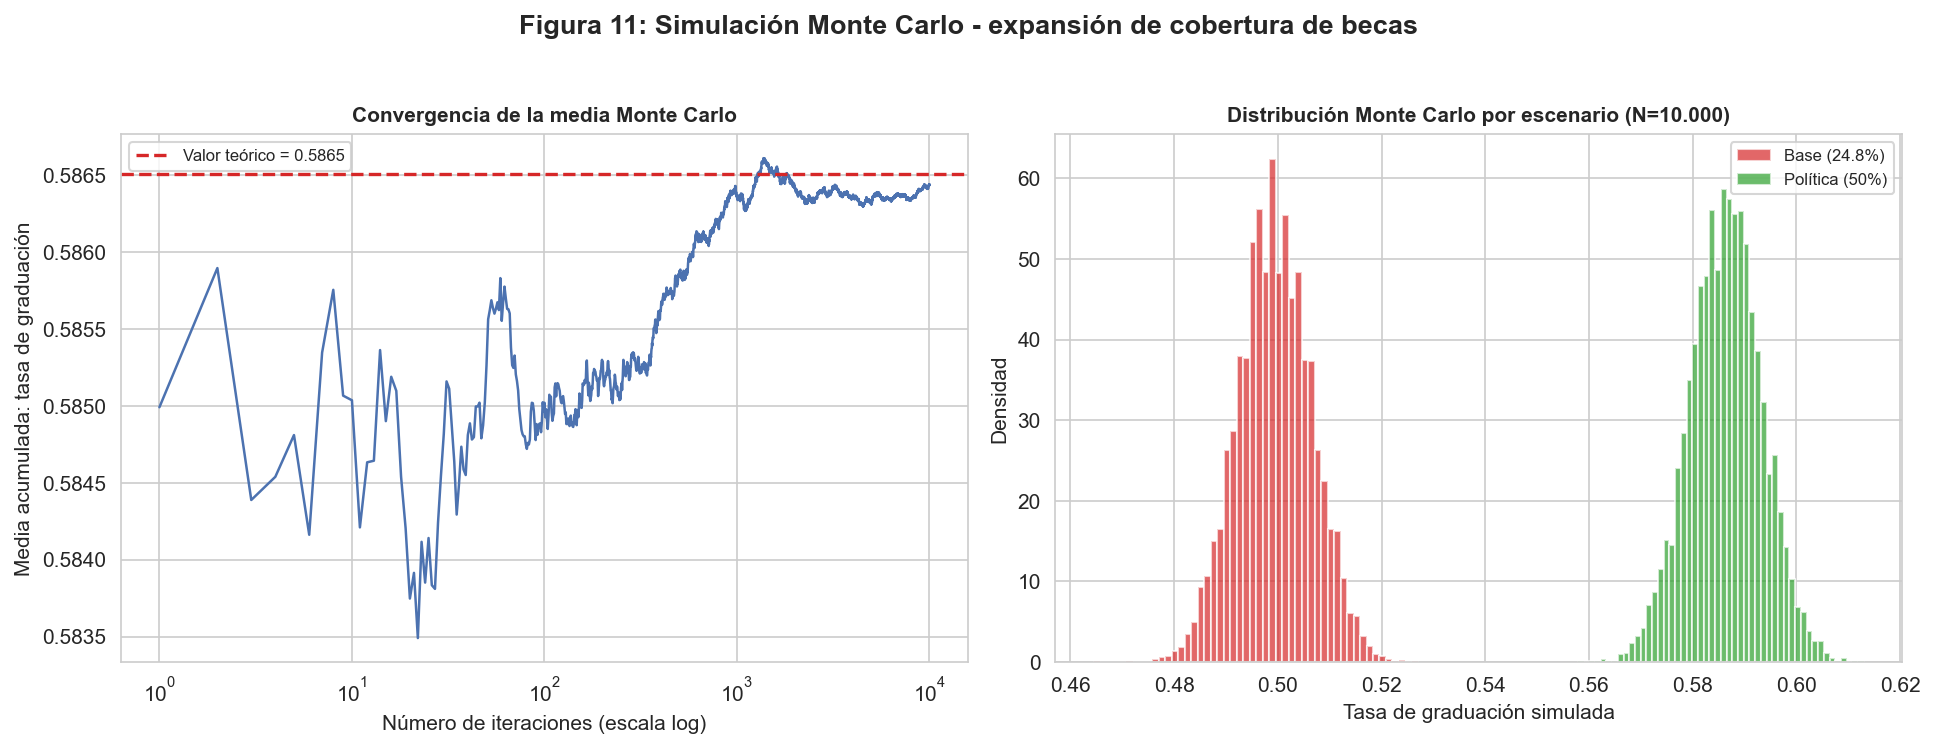
\includegraphics[width=0.95\textwidth]{fig11_montecarlo_becas.png}
\caption{Izquierda: convergencia de la media acumulada de la tasa de graduación hacia el valor
teórico (0.5865). Derecha: distribuciones Monte Carlo por escenario.}
\label{fig:mc}
\end{figure}

La media acumulada converge al valor teórico poblacional (0.58651) con un error estándar
Monte Carlo de $7.0\times10^{-5}$ en $N=10{,}000$: el ruido de simulación es varios órdenes de
magnitud menor que el efecto estimado, confirmando que el mínimo exigido de iteraciones es más
que suficiente. Duplicar la cobertura de becas se asocia a un incremento esperado de
\textbf{8.7 p.p.\ en graduación} y una reducción de \textbf{6.7 p.p.\ en deserción},
cuantificando la recomendación cualitativa de S1. La interpretación causal debe ser cautelosa:
el resultado es una cota superior orientativa, útil para justificar un piloto controlado que
permita estimar el efecto causal real en la Sumativa 3.

\section{Análisis de robustez}

\begin{conexionbox}
S1 reportó estimaciones puntuales (Tabla 3) y pruebas de hipótesis (Sección 4) sin evaluar
formalmente su sensibilidad a observaciones atípicas. Esta sección las somete a jackknife,
\textit{winsorizing} y una prueba no paramétrica alternativa.
\end{conexionbox}

Para cada observación $i$ se calcula su influencia jackknife sobre la media,
$\text{infl}_i=n(\bar{X}-\bar{X}_{(-i)})$.

\begin{figure}[h!]
\centering
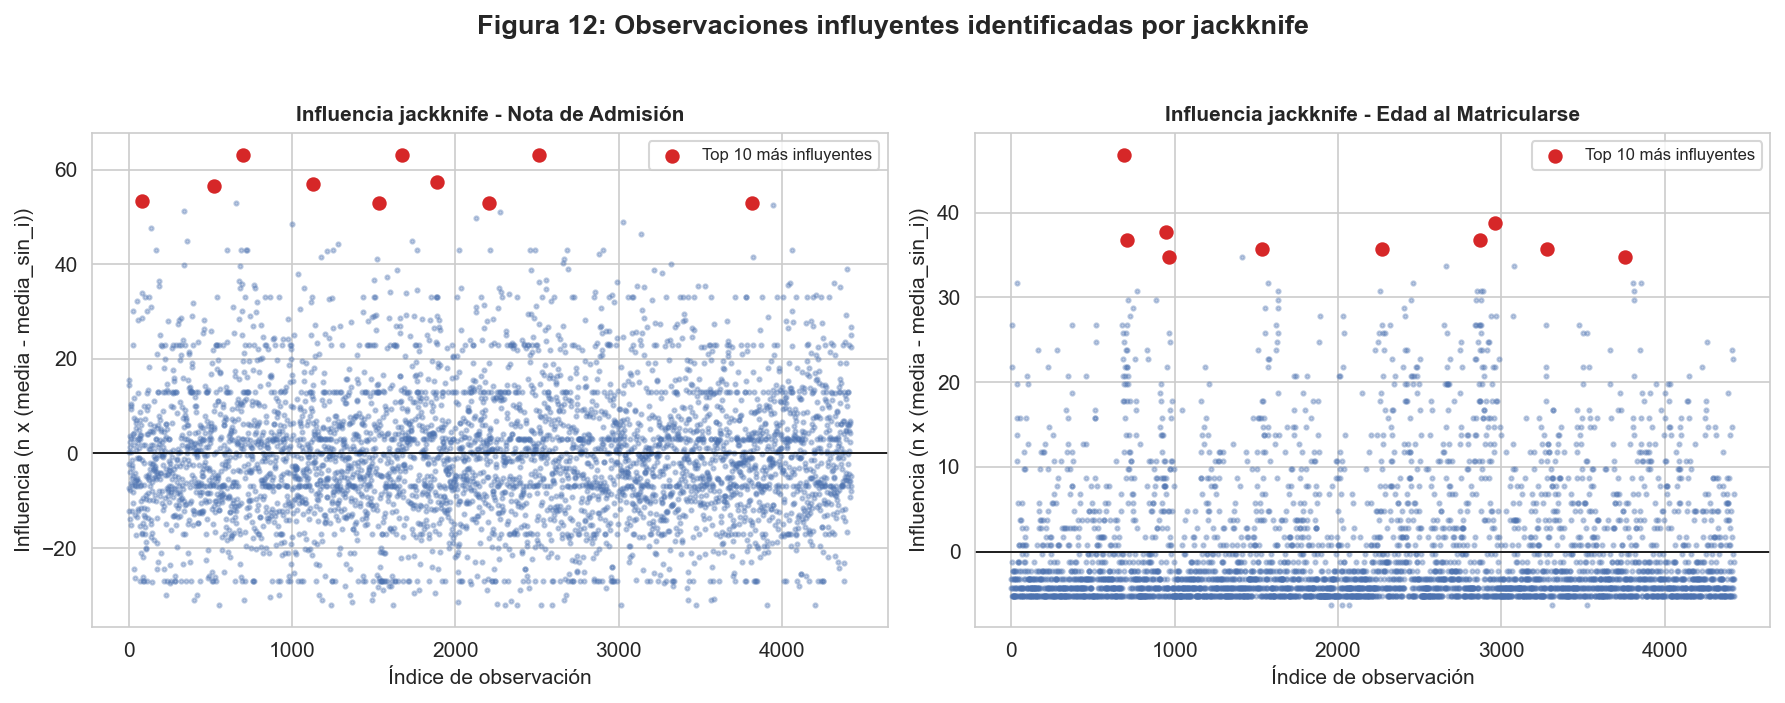
\includegraphics[width=0.95\textwidth]{fig12_jackknife_influencia.png}
\caption{Influencia jackknife por observación: Nota de Admisión y Edad al Matricularse.}
\label{fig:jack}
\end{figure}

Las observaciones más influyentes en \textbf{Nota de Admisión} son notas en el techo de escala
(190.0, máximo del sistema ENES); en \textbf{Edad}, estudiantes de 60 a 70 años. Ninguna es un
error de captura (son valores válidos) por lo que no corresponde eliminarlas, pero sí
documentarlas como fuente de heterogeneidad. Al winsorizar la Prueba 1 al 1\,\%/99\,\%, el
resultado se mantiene ($t=-7.923$, $p=3.28\times10^{-15}$ vs.\ original $t=-7.657$,
$p=2.59\times10^{-14}$): la decisión de rechazo no cambia. Mann-Whitney $U$ (alternativa no
paramétrica, sin asumir normalidad) confirma la Prueba 1 ($U=1{,}326{,}633.5$,
$p=3.25\times10^{-15}$, rank-biserial $r=0.155$): la conclusión sustantiva no depende del
supuesto de normalidad violado por \textit{Graduate}.

Para \textbf{Edad}, la asimetría (+2.05) es crítica: media $=23.265$ (IC clásico
$[23.041,23.489]$), media recortada al 10\,\% $=21.574$, mediana $=20.000$ con IC bootstrap al
95\,\% \textbf{degenerado en $[20.000,20.000]$}. La alta concentración de estudiantes entre 18
y 20 años hace que casi cualquier remuestra bootstrap reproduzca exactamente la mediana
observada, mientras la media desplazada por una cola pequeña pero muy influyente de
estudiantes adultos, según el jackknife se ubica más de tres años por encima: es una
estimación puntual precisa que no representa bien al ``estudiante típico''. La correlación
Edad-Resultado es estable ante la remoción del 1\,\% superior de edades ($r=-0.243\to-0.257$,
43 observaciones removidas).

\textbf{Síntesis crítica}: son \emph{robustos sin reservas} la diferencia de nota de admisión
Dropout/Graduate (cuatro verificaciones concordantes: Welch, permutación, winsorizing y
Mann-Whitney), las correlaciones de las notas semestrales, y la asociación beca-resultado.
\emph{Requieren cautela}: la media de Edad al Matricularse (reportar junto con la mediana) y
el parámetro PIB, cuya dependencia por cohortes ningún método de remuestreo a nivel de
observación individual logra resolver.

\section{Preparación de insumos para la Sumativa 3}

\begin{conexionbox}[Conexión con la Sumativa 3]
S1 propuso como próximo paso el modelamiento predictivo multiclase. Esta sección consolida el
reporte de resultados validados que constituye la entrada directa para ese modelamiento.
\end{conexionbox}

\begin{table}[h!]
\centering
\small
\begin{tabular}{lrl}
\toprule
\textbf{Parámetro} & \textbf{Media} & \textbf{Estado de validación} \\
\midrule
Nota de Admisión        & 126.978 & Robusto (IC clásico $\equiv$ BCa) \\
Edad al Matricularse    & 23.265  & Robusto en media; usar mediana (20.0) como complemento \\
Nota 1\textsuperscript{er} Semestre & 10.641 & Robusto (IC clásico $\equiv$ BCa) \\
PIB                     & 0.002   & Con cautela: dependencia por cohortes no resuelta \\
\bottomrule
\end{tabular}
\caption{Parámetros robustamente estimados.}
\label{tab:resumen_param}
\end{table}

\vspace{-0.6em}
\begin{table}[h!]
\centering
\small
\begin{tabular}{lrl}
\toprule
\textbf{Correlación con resultado} & \textbf{$r$} & \textbf{Clasificación} \\
\midrule
Nota 2\textsuperscript{do} Semestre & 0.567 & Robusta y de relevancia práctica alta \\
Nota 1\textsuperscript{er} Semestre & 0.485 & Robusta y de relevancia práctica alta \\
Edad al Matricularse                & $-$0.243 & Robusta, relevancia moderada \\
Nota de Admisión                    & 0.121 & Robusta, relevancia baja \\
PIB                                 & 0.044 & Estable pero marginal usar con cautela\\
\bottomrule
\end{tabular}
\caption{Correlaciones estables identificadas mediante bootstrap.}
\label{tab:resumen_corr}
\end{table}

\textbf{Observaciones influyentes:} notas de admisión en el techo de escala (=190) y
estudiantes de 60 a 70 años; ambos grupos son válidos y ameritan tratamiento diferenciado (por
ejemplo, una variable indicadora de ``estudiante adulto'') en el modelamiento de S3.
\textbf{Pruebas validadas:} diferencia en nota de admisión (Welch, permutación y Mann-Whitney
concordantes) y asociación beca-resultado ($\chi^2$ y permutación concordantes, Cramér's
$V=0.30$). \textbf{Simulación validada:} expansión de cobertura de becas al 50\,\% asociada a
$+8.7$ p.p.\ en graduación y $-6.7$ p.p.\ en deserción, bajo el supuesto (no causal) de
transportabilidad.

\textbf{Recomendaciones metodológicas para S3:} 

\begin{enumerate}
    \item Reportar la mediana junto con la media de
Edad al Matricularse dada su asimetría
    \item Excluir o agregar por cohorte el PIB antes de
usarlo como predictor individual
    \item Priorizar las notas semestrales como variables
predictoras centrales del modelo multiclase
    \item  Tratar la beca como variable de
intervención, no solo predictiva --requiere diseño cuasi-experimental antes de decisiones de
política institucional
    \item Conservar, no eliminar, las observaciones influyentes identificadas
    \item Mantener el protocolo de validación cruzada $k=5$ de S1, incorporando una validación por bootstrap del desempeño del modelo final.
\end{enumerate}

El notebook \texttt{\href{https://github.com/dark452/mcdi501-grupo1/blob/main/notebooks/F3.ipynb}{notebooks/F3.ipynb}},
disponible en el repositorio GitHub de la portada, reproduce íntegramente estos análisis --con
funciones documentadas de bootstrap, permutación, Monte Carlo y jackknife, semilla
\texttt{seed=42} y genera automáticamente las cinco figuras de este informe.


\begin{thebibliography}{99}
\bibitem[Efron \& Tibshirani(1993)]{efron1993}
Efron, B., \& Tibshirani, R. J. (1993). \textit{An introduction to the bootstrap}. Chapman \& Hall/CRC.

\bibitem[McKinney(2022)]{mckinney2022}
McKinney, W. (2022). \textit{Python for data analysis} (3rd ed.). O'Reilly Media.

\bibitem[Montgomery \& Runger(2018)]{montgomery2018}
Montgomery, D. C., \& Runger, G. C. (2018). \textit{Applied statistics and probability for engineers} (7th ed.). Wiley.

\bibitem[Realinho et al.(2022)]{realinho2022}
Realinho, V., Machado, J., Baptista, L., \& Martins, M. V. (2022). Predicting student dropout and academic success. \textit{Data}, \textit{7}(11), 146. \url{https://doi.org/10.3390/data7110146}

\bibitem[Walpole et al.(2012)]{walpole2012}
Walpole, R. E., Myers, R. H., Myers, S. L., \& Ye, K. (2012). \textit{Probabilidad y estadística para ingeniería y ciencias} (9.ª ed.). Pearson.
\end{thebibliography}
\end{document}
